\documentclass[12pt]{scrartcl} % se puede cambiar por article
\RequirePackage{amsmath,amsfonts,amssymb,amsthm}
\usepackage{eulervm} % tipografía con soporte para matemáticas
\usepackage{caption}

\usepackage{exercise}
\usepackage{graphicx}
\DeclareMathOperator*{\argmax}{argmax}

\usepackage[utf8]{inputenc}
\usepackage[spanish,mexico]{babel}
% sgamex.sty from Rubinstein
\usepackage{sgamex}

\usepackage{setspace}
\onehalfspacing % doble espacio: \doublespacing

\title{Solución de la tarea 2a}
\author{Emmanuel Alcalá}
\date{\today}

\begin{document}
\maketitle

% Respuestas enumeradas con paquete Exercise
\begin{Exercise}[name={Respuesta}]
  1.
  \begin{center}
    \centering
    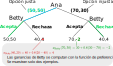
\includegraphics[width=0.75\textwidth]{tarea2b_p1.png}
  \end{center}
  2. El ENPS es $ \{50/50_{\text{O justa}}, (Acepta, rechaza)\} $ con ganancias $ (50, 50) $.

\end{Exercise}

\begin{Exercise}[name={Respuesta}]

  El juego es de información incompleta. El subjuegos de la segunda etapa debe resolverse de forma simultánea. Comenzando con inducción hacia atrás.

  \begin{center}
    \begin{game}{3}{3}[E1][E2]
      &   L            &   M   &   H \\
      L   &  -50, 300  &   0,325  &   50,250\\
      M   &  -25,350   &  50,400  &  150,325\\
      H   &  -100,400  & -25,500  &  100,450
    \end{game}
  \end{center}

  Para E1, M domina a H, y para E2, M domina a L. Por lo que queda el juego reducido

  \begin{center}
    \begin{game}{3}{3}[Jugador 1][Jugador 2]
      &   M   &   H \\
      L   &   0,325  &   50,250\\
      M   &  \textbf{50,400}  &  150,325
    \end{game}
  \end{center}

  Según el algoritmo de tres pasos, en negritas se encuentra el par de ganancias que maximizan, por lo que (M, M) constituye un EN, con ganancias (50, 400).

  sustituimos las ganancias en el nodo terminal de E2 cuando elige E, y comparamos la utilidad de elegir E con la de elegir NE, y vemos que conviene E. El ENPS es entonces $ \{(E, M), M\} $ con ganancias en equilibrio $ (50, 400) $.



\end{Exercise}

\end{document}

